% !TEX root = ./Research_and_SA.tex

% FROM THE NIH SITE:
% Is the proposed research project of high scientific quality, and is it well integrated with the proposed research training plan?
% Based on the sponsor’s description of his/her active research program, is the applicant’s proposed research project sufficiently distinct from the sponsor’s funded research for the applicant’s career stage?
% Is the research project consistent with the applicant’s stage of research development?
% Is the proposed time frame feasible to accomplish the proposed training?

%\textbf{SIGNIFICANCE}\\
\subsubsection*{SIGNIFICANCE}
RNA lies at the center of cellular function. Its most appreciated role is to carry protein blueprints to the ribosome for manufacture.
Only recently have researchers begun to appreciate its myriad of other functions, many of which also lie at the center of important cellular processes and are implicated in a variety of disease states \cite{CechNoncodingRNARevolution2014,DellaRagioneNoncodingRNAschromatin2014,AnastasiadouNoncodingRNAnetworks2018}.
Long noncoding RNA (lncRNA) comprise one such important class of RNA that does not participate in the central dogma \cite{RinnGenomeRegulationLong2012}. Alarmingly, the human genome encodes for as many lncRNA as proteins \cite{Rinntranscriptionalactivityhuman2003,RinnGenomeRegulationLong2012}.
These transcripts are typically greater than 200 bases, and participate in binding both proteins and nucleic acids, often both at the same time \cite{AnastasiadouNoncodingRNAnetworks2018,RinnGenomeRegulationLong2012}.
In a striking example, \textit{SNGH5} is a long noncoding RNA (lncRNA) of largely unknown function, that that has been linked to cancer cell survival and metastasis in a diversity of different cancers from leukemias to melanoma \cite{TanakaRitsukoIntronicU50small2001,DamasSNHG5promotescolorectal2016,ZhaoLongnoncodingRNA2016,HeLncRNASNHG5regulates2017,YanSNHG5promotesproliferation2018,MalncRNASNHG5associated2018,ShenLncRNASNHG5miR26a2018,ZhengLongnoncodingRNA2018}.
This 2 kilobase transcript localizes to the cytoplasm and is upregulated in these disease states.
\textit{SNGH5} has been implicated to interact with a variety of mRNAs to control expression, though little else is known about its role in normal cell function.
Where and when does \textit{SNGH5}, and other similar lncRNA, interact with their mRNA targets?
How long do these interactions occur, and what other cellular machinery is present?
Despite such burning questions in the field of lncRNA, a tool to directly image these species and their interacting partners in living cells has yet to be reported. \textit{Herein, I propose a robust imaging tool for multicomponent, single-molecule visualization of RNA dynamics in living cells.}

\subsubsection*{BACKGROUND}
%%%%%%%%%%%%%%%%%%%%%%%%%%%%%%%%%%%%%%%%%%%%%%%%%%%%%%%%%%%%%%%%%%%%%%%%%%%%%%%%
%Riboglow
\begin{wrapfigure}[29]{R}{7.5cm}
\vspace{-0.2in}
\begin{centering}
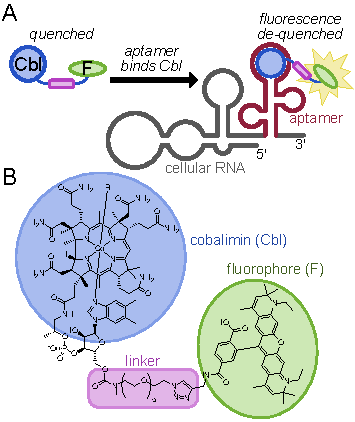
\includegraphics[width=\textwidth]{figures/fig1v3.pdf}
\end{centering}
\footnotesize
\caption{\label{figure:riboglow}
A) Cobalamin acts as a quenching and localization moiety to guide a fluorescent probe to an RNA transcript of interest. When unbound, fluorescence is quenched. In the presence of RNA tagged with the cobalamin riboswitch, fluorescence is restored. B) Structure of the generation 1 Riboglow probe. A polyethylene glycol linker of five units (5xPEG) connected to the 5' hydroxly of the cobalamin ribose was used to tether an ATTO 590 fluorophore to the construct.
}
\end{wrapfigure}
%%%%%%%%%%%%%%%%%%%%%%%%%%%%%%%%%%%%%%%%%%%%%%%%%%%%%%%%%%%%%%%%%%%%%%%%%%%%%%%%

Protein studies benefit from a large imaging toolkit that has been developed over the last 25 years. Genetically encodable fluorescent proteins are now ubiquitous for the study of the localization of any translated target in the cell. While fluorescent proteins are a mature, well-understood technology, tools for imaging the localization of individual RNA transcripts in living cells remain limited. The most popular systems to date include dye-binding aptamers (Spinach \cite{PaigeRNAMimicsGreen2011}, Broccoli \cite{FilonovBroccoliRapidSelection2014}, and Mango \cite{AutourFluorogenicRNAMango2018,DolgosheinaRNAMangoAptamerFluorophore2014}), and RNA-binding protein fusions (MS2-FPs) \cite{FuscoSinglemRNAMolecules2003,TutucciimprovedMS2system2018}.

The most analogous to fluoresecent proteins, dye-binding aptamers utilize exogenously administered dyes that give fluorescence induction upon binding their RNA partner  \cite{PaigeRNAMimicsGreen2011,FilonovBroccoliRapidSelection2014,AutourFluorogenicRNAMango2018,DolgosheinaRNAMangoAptamerFluorophore2014}.
This sequence is encoded downstream of an RNA of interest to track its location in the cell. Though excellent binders for their dyes, the aptamers utilized by this technology are unstable in mammalian cells due to their nonnative structure \cite{EtzelSyntheticRiboswitchesPlug2017,IiiStructuralbasishighaffinity2017,WarnerStructuralbasisactivity2014,JengFluorophoreligandbinding2016}.
Additionally, though fluorescence turn-on is excellent \textit{in vitro}, often reaching 1,000 fold, signal induction in cells is typically two to four fold, most likely due to nonspecific binding of the dye, making them poor probes for single-molecule tracking \cite{AutourFluorogenicRNAMango2018}.

RNA-binding protein fusions are a much more robust technique for imaging RNA transcripts  \cite{FuscoSinglemRNAMolecules2003}. This method often utilizes the MS2 bacteriophage coat protein that binds an encoded stem loop of RNA. When MS2 is fused to a fluorescent protein, transcripts can be visualized in the cell. In order to concentrate the fluorescence signal above background, multiple stem loops are placed in series (up to 24 in a row). Though this technique has enabled imaging of single transcripts in the cell  \cite{MorisakiRealtimequantificationsingle2016,FuscoSinglemRNAMolecules2003}, the resulting protein-RNA complex is prohibitively large for many studies \cite{TutucciimprovedMS2system2018}.

Riboglow is a recently developed platform in the Palmer lab that solves many of the drawbacks of current RNA imaging techniques (Figure \ref{figure:riboglow}) \cite{BraselmannDevelopmentriboswitchbasedplatform2017}. The two-component system utilizes a synthetic fluorophore-quencher pair, and a genetically-encoded riboswitch. A transcript of interest is first tagged within the cell, and the probe construct is administered via bead loading \cite{McNeilGlassbeadsload1987,Hayashi-TakanakaTrackingepigenetichistone2011,MorisakiRealtimequantificationsingle2016}.
When the construct binds the transcribed riboswitch, the fluorophore is dequenched, giving fluorescent signal. Like the dye-binding aptamers, Riboglow utilizes a riboswitch receptor domain that natively binds vitamin B\textsubscript{12} (cobalamin, Cbl, Figure \ref{figure:riboglow}B) \cite{JohnsonJrB12cofactorsdirectly2012}.
Conveniently, cobalamin is known to act as a fluorescence quencher for a variety of fluorophores \cite{RosendahlSynthesisbiologicalactivity1982,LeeDesignSynthesisCharacterization2009,SmeltzerSynthesisCharacterizationFluorescent2001}.
With Riboglow, the cobalamin center is conjugated to the fluorophore through a flexible linker that promotes quenching in the unbound state, but enables the fluorophore to reside at a distance in the bound state (Figure \ref{figure:riboglow}B).

The Palmer lab found that this initial generation of Riboglow has the potential to outperform the existing tools in the field.
Its use of a naturally-occurring riboswitch imparts stability to the construct that is not present in aptamer-based techniques \cite{PorterRecurrentRNAmotifs2017}.
Additionally, the use of a donor-quencher pair reduces nonspecific fluorescence in the unbound state. Such signal induction is low in the aptamer-binding dyes, and cannot be obtained at all with the MS2-fluorescent protein fusions. Due to these advantages, Riboglow outperformed Broccoli and the MS2 system in initial studies of mRNA stress granule (SG) localization in mammalian cells.

Though promising, the initial iteration of Riboglow has significant room for improvement. With initial constructs, signal induction upon riboswitch binding never exceeded seven fold \textit{in vitro}, and the pendant dye was never fully quenched (with 10-20\% residual fluorescence) \cite{BraselmannDevelopmentriboswitchbasedplatform2017}. Additionally, to effectively detect stress granules, four riboswitches had to be placed in series to concentrate fluorescence signal \cite{BraselmannDevelopmentriboswitchbasedplatform2017}. This high background precluded single-molecule imaging. Finally, the strategy cannot currently be used to monitor the location of multiple transcripts in tandem. Herein, I will propose strategies to overcome these limitations through simultaneous modulation of the small molecule construct and riboswitch sequence. This is an undertaking for which I am uniquely suited, due to my experience of tandem modification of small molecule-protein interactions during my graduate studies. First, I will synthesize a variety of new Riboglow probes to optimize fluorescence quenching (Aim 1). Next, I will turn to the structure of the riboswitch itself. A screen for brightness will select the best riboswitch sequence to match the optimized cobalamin probe (Aim 2). This new, brighter pair will be tested for single-molecule detection. Finally, I will use SELEX to identify mutually orthogonal probe-riboswitch pairs for multicomponent RNA imaging, and will test these new tools by tracking lncRNA-mRNA interactions in living cells (Aim 3).

\subsubsection*{APPROACH \underline{Aim 1.} Synthesize improved Riboglow probes.}
%%%%%%%%%%%%%%%%%%%%%%%%%%%%%%%%%%%%%%%%%%%%%%%%%%%%%%%%%%%%%%%%%%%%%%%%%%%%%%%%
%Cbl constructs
\begin{wrapfigure}{r}{10cm}
\vspace{-0.13in} % this is the happy medium between top of fig and bottom...
\begin{centering}
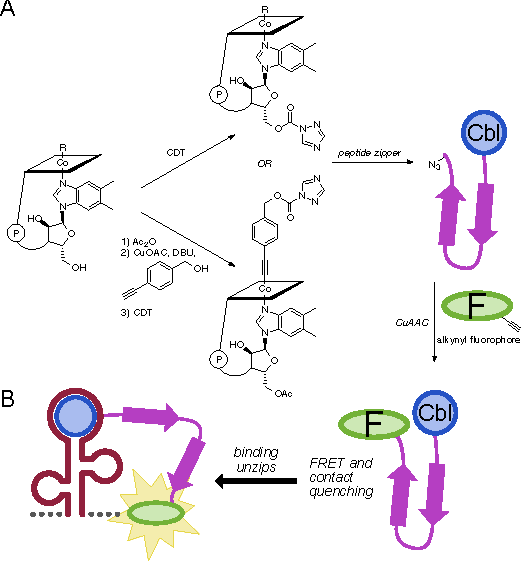
\includegraphics[width=\textwidth]{figures/aim1v5.pdf}
\end{centering}
\footnotesize
\caption{\label{figure:CblConstructs}
A) Synthesis of two structurally distinct attachment points for Riboglow probes. Both modes of conjugation have already been described in Ref. \cite{ChrominskiVitaminB12Derivatives2014} (see Gryko support letter). Top: Conjugation with CDT at the ribose 5' OH was used in the first-generation probes \cite{BraselmannDevelopmentriboswitchbasedplatform2017}. Bottom: Alkynylation at the metal center with 4-ethynylbenzyl alcohol will enable subsequent coupling with CDT. Ac\textsubscript{2}O: acetic anhydride, DBU: 1,8-diazabicyclo[5.4.0]undec-7-ene, CDT: 1,1′-carbonyl-di-(1,2,4-triazole), CuAAC: copper catalyzed azide-alkyne cycloaddition. B) Tryptophan zipper peptides will be used to maximize FRET and contact quenching in the unbound state.
}
\end{wrapfigure}
%%%%%%%%%%%%%%%%%%%%%%%%%%%%%%%%%%%%%%%%%%%%%%%%%%%%%%%%%%%%%%%%%%%%%%%%%%%%%%%%

The main drawback of Riboglow is the poor turn-on that is observed upon probe binding. In this aim, I intend to leverage my background in synthetic chemistry to produce a panel of diverse probe structures that improve fluorescence quenching (and thus signal induction). In previous studies in collaboration with Professor Dorota Gryko (see Gryko letter of support) a small number of linkers and fluorophores were evaluated for quenching and fluorescence turn-on. Linker length and fluorophore wavelength were varied to gauge the quenching ability of cobalamin. Remarkably, some degree of quenching occurred in all of the constructs synthesized, regardless of the spectral overlap of the fluorophore and the cobalamin. However, most retained 10-20\% residual fluorescence, which increased background signal significantly. \textit{To optimize probe function, I will vary linker composition, attachment point, and pendant fluorophore with the goal of obtaining 98\% quenching in vitro.}

%%%%%%%%%%%%%%%%%%%%%%%%%%%%%%%%%%%%%%%%%%%%%%%%%%%%%%%%%%%%%%%%%%%%%%%%%%%%%%%%
%Zipper Linkers
\begin{wraptable}{L}{9cm}
\vspace{-0.13in} % this is the happy medium between top of fig and bottom...
\caption{Tryptophan zippers of varying stability will be tested to maximize fluorescence quenching. Azidoalanine (Az) will be added to the C-terminus to enable easy fluorophore conjugation. Values were obtained from ref.\ \cite{FesinmeyerEnhancedHairpinStability2004} and reflect measurements for the peptide without the C-terminal azidoalanine.}\label{table:ZipperLinkers}
\begin{tabular}{c | c >{\centering\arraybackslash}m{1.5cm} } % funky greater than thing centers wrapped text in the cell
\toprule
Sequence & Tm ($^\circ$C) &  \% folded (25 $^\circ$C) \\\toprule
\texttt{KKWTW-NPATGK-WTWQE(Az)} & 85 & >96 \\ % \texttt{} makes things monospace
\texttt{KKYTW-NPATGK-WTVQE(Az)} & 66 & 92 \\
\texttt{GEWTY-NPATGK-FTVTE(Az)} & 47 & 74 \\  \hline
\texttt{GGGGG-GGGGGG-GGGGG(Az)} & N/A & N/A \\
\bottomrule
\end{tabular}
\end{wraptable}
%%%%%%%%%%%%%%%%%%%%%%%%%%%%%%%%%%%%%%%%%%%%%%%%%%%%%%%%%%%%%%%%%%%%%%%%%%%%%%%%

Ideally, in the unbound state, the cobalamin and fluorophore would be closely associated to maximize FRET and contact quenching \cite{RosendahlSynthesisbiologicalactivity1982,ShellVitaminB12Tunable2015,ShellTunableVisibleNearIR2014}.
In the RNA-bound state, the molecules would reside at their maximal distance to promote fluorescence \cite{LeeDesignSynthesisCharacterization2009}.
To strike this balance, I will use a synthetic $\upbeta$-hairpin as the linker between cobalamin and the fluorophore (Figure \ref{figure:CblConstructs}B, Table \ref{table:ZipperLinkers}).
A number of such $\upbeta$-hairpins have been developed, and are referred to as tryptophan zippers \cite{CochranTryptophanzippersStable2001}.
These motifs are as small as twelve amino acids and some are stable to denaturation up to 85 $^\circ$C (Table \ref{table:ZipperLinkers}).
In the unbound state, such a linker would hold the quencher and fluorophore in close proximity (due to the short distance between the N and C-termini of the peptide, Figure \ref{figure:CblConstructs}B).
When the cobalamin is bound by the riboswitch, steric occlusion would force the $\upbeta$-hairpin to unfold and place the fluorophore-quencher pair at a larger distance.
A wide range of tryptophan zippers have been developed with a variety of structures and stabilities, enabling easy construction of a range of different linkers via solid phase peptide synthesis \cite{CochranTryptophanzippersStable2001,KierProbingLowerSize2008,AndersenMinimizationOptimizationDesigned2006,FesinmeyerEnhancedHairpinStability2004} (see Equipment document).
To enable modularity, an azidoalanine amino acid will be appended to the C-termini of all linkers during peptide synthesis.
Cobalamin will then be coupled to the linker via amide coupling and alkynyl fluorphores will be appended via copper catalyzed azide-alkyne cycloaddition (CuAAC, Figure \ref{figure:CblConstructs}A) \cite{KolbHartmuthC.ClickChemistryDiverse2001,PattersonFindingRightBioorthogonal2014}.
This general synthetic sequence is very similar to that used to make the original Riboglow probes \cite{BraselmannDevelopmentriboswitchbasedplatform2017}.
A starting set if linkers are listed in Table \ref{table:ZipperLinkers}.
The polyglycine linker will be used as a negative control for a sequence with little secondary structure, but identical length.
If the zipper folds prove to be too stable (dequenching is not observed), the amino acids will be varied to tune the melting temperature.
Or, if adequate quenching is not observed, the relative positions of the N and C-termini will be adjusted based upon structural data available in the Protein Data Bank (PDB) \cite{AndersenMinimizationOptimizationDesigned2006}.
All newly synthesized Riboglow probes will be purified via high-performance liquid chromatography (HPLC), and structurally verified via nuclear magnetic resonance (NMR) spectroscopy and high resolution mass spectrometry (HRMS).
Each new construct will be tested for its ability to quench fluorescence in vitro by comparing the fluorescence of the construct with that of the free fluorophore in solution. Fluorescence signal in the presence of the Riboglow riboswitch will also be measured to calculate fluorescence turn-on.

Another underexplored variable of the original Riboglow probes is the linker attachment point.
Though the 5' hydroxyl of the cobalamin ribose is the most accessible nucleophile on the structure, there exist several other possible sites of conjugation.
Perhaps the second most common site is the axial ligand of the cobalt metal itself.
Though many studies have taken advantage of the labile nature of certain alkyl modifications at this position \cite{ShellVitaminB12Tunable2015}, others have found alkynyl modifications to be stable to air and light \cite{ChrominskiReductionfreesynthesisstable2013,RuetzMarkusPhenylethynylcobalaminLightStable2013}.
Following this precedent, I will synthesize a cobalamin with an alkyne handle attached to the cobalt metal center (Figure \ref{figure:CblConstructs}A, Bottom).
Such a molecule has already been synthesized in the lab of Professor Dorota Gryko (see Gryko letter of support), and shown to be amenable to functionalization \cite{ChrominskiVitaminB12Derivatives2014}.

These constructs will also be evaluated for degree of fluorescence quenching, and brightness in the presence and absence of the cobalamin riboswitch.
It is possible that incorporation of a ligand at this site on the metal center will abolish binding to the native riboswitch due to its positioning in the binding pocket \cite{JohnsonJrB12cofactorsdirectly2012}.
If this is the case, these probes could serve as excellent starting points for directed evolution of orthogonal aptamer-probe pairs (see Aim 3).
Additionally, perturbations to the native binding mode of cobalamin could reduce off-target association with native B\textsubscript{12} machinery \cite{PathareSynthesisCobalaminBiotin1996}, further reducing fluorescence background.

\begin{wraptable}{R}{10cm}
\vspace{-0.13in} % this is the happy medium between top of fig and bottom...
\caption{
A range of fluorophores will be explored for optimal quenching and signal induction. Cy5 and the ATTO series were utilized in the first generation Riboglow system, and will also be used here with new linkers and Cbl attachment points. Photophysical values were obtained from Atto tec and refs.\ \cite{BraselmannDevelopmentriboswitchbasedplatform2017} and  \cite{Grimmgeneralmethodfinetune2017}.
$\lambda$: wavelength, $\epsilon$: extinction coefficient, $\phi$: quantum yield.
}\label{fluorophores}
\begin{tabular}{c|cccc}
  \toprule
 Dye &  $\lambda$\textsubscript{ex} (nm) &  $\lambda$\textsubscript{em} (nm) &  $\epsilon$ (M\textsuperscript{-1}cm\textsuperscript{-1}) &  $\phi$ \\\toprule
Cy5 & 646 & 662 & 271,000 & 0.2\\
ATTO 488 & 501 & 523 & 90,000 & 0.8\\
ATTO 590 & 594 & 624 & 120,000 & 0.8\\
ATTO 633 & 629 & 657 & 130,000 & 0.6\\  \hline
\textbf{JF\textsubscript{549}} & \textbf{549} & \textbf{571} & \textbf{101,000} & \textbf{0.88}\\ % this is a painful solution, with more time try this?: https://tex.stackexchange.com/questions/309833/format-whole-row-of-table-as-bold
\textbf{JF\textsubscript{585}} & \textbf{585} & \textbf{609} & \textbf{156,000} & \textbf{0.78}\\
\textbf{JF\textsubscript{635}} & \textbf{635} & \textbf{652} & \textbf{167,000} & \textbf{0.56}\\
\bottomrule
\end{tabular}
\end{wraptable}

The final variable in the molecular structure of the Riboglow probe is the fluorophore itself. The ideal probe would minimize cellular autofluorescence through the use of a red fluorophore with a high extinction coefficient. The Janelia Fluor series of dyes is well suited for this application \cite{Grimmgeneralmethodfinetune2017,Grimmgeneralmethodimprove2015}. With minor modifications to the rhodamine scaffold, Janelia Fluors have varying excitation and emission spectra, and excellent photophysical properties.
Table \ref{fluorophores} includes a subset of the probes that will be explored.
Emphasis will be placed on fluorophores with high extinction coefficients ($\epsilon$) and quantum yields ($\phi$), with the intent for these probes to be used in single-molecule imaging (Aim 2).
Additionally, JF\textsubscript{585} and JF\textsubscript{635} were shown to be highly fluorogenic upon conjugation to a protein tag, with absorbance increases of 80 and 113-fold respectively \cite{Grimmgeneralmethodfinetune2017}.
The Lavis lab makes these probes freely available, and has offered (personal communication) to provide us with alkynylated versions for easy conjugation via CuAAC (Figure \ref{figure:CblConstructs}A).
Probes containing these new fluorophores will be evaluated as previously described, with the addition of a test for fluorophore photostability.
Stability under extended illumination will be important for single-molecule localization (Aim 2), thus these experiments will give an additional point of comparison for probe quality.

\textbf{Expected Outcomes and alternate approaches:}\\
To identify probes with improved quenching and fluorescence turn-on, linker, attachment point, and fluorophore will be varied. To start, I will target 98\% fluorescence quenching \textit{in vitro}. With four linkers, two attachment points, and seven fluorophores, 56 constructs are possible. Though not all of these will be evaluated, simple chemistries involving amide bond couplings and click chemistry will enable us to sample a large amount of this structure space in a rapid fashion. If $\upbeta$-hairpin zippers do not yield improvements in quenching, other linkers with varying rigidity and lengths will be explored \cite{LeeDesignSynthesisCharacterization2009}, specifically those that promote direct contact between the fluorophore and the cobalamin. Also, it should be noted that new cobalamin constructs are not necessary for the success of aims 2 or 3. It is likely that all three aims will be pursued in parallel, with new discoveries in each informing project direction.

\subsubsection*{\underline{Aim 2.} Adapt Riboglow for single-molecule imaging.}
Visualization of the lifecycle of single RNA transcripts as they move throughout the cell remains a holy grail of RNA imaging \cite{LiCentraldogmasinglemolecule2011}.
This is an entirely feasible goal due to the fact that so few copies of an individual RNA transcript exist in a cell at any given time (the samples are by definition sparsely populated) \cite{CabiliLocalizationabundanceanalysis2015,LiCentraldogmasinglemolecule2011,AndreckaSinglemoleculetrackingmRNA2008}.
Though several recent studies have demonstrated visualization of individual mRNA transcripts, all have required the use of at least 24 repeats of the MS2-binding stem loop \cite{KatzMappingtranslationhotspots2016,FuscoSinglemRNAMolecules2003,YamagishiSinglemoleculeimagingvactin2009,HalsteadRNAbiosensorimaging2015}.
When these loops (which each bind two MS2 proteins) are fully populated, a complex of more than 2,000 kilodaltons is produced.
Such a structure is several times larger than most mRNA, giving the potential to perturb normal mRNA behavior.
Riboglow reduces the size of the fluorescent probe by 10--100-fold (relative to the MS2 system), however, high fluorescence background and poor signal induction precluded single-molecule studies \cite{BraselmannDevelopmentriboswitchbasedplatform2017}.

With the wide variety of new probe constructs developed to optimize quenching (Aim 1), changes will be made to the sequence of the cobalamin riboswitch with the goal of increasing fluorescence turn-on by 50-fold. \textit{A directed evolution screen for fluorescence brightness will identify optimal riboswitch sequences that promote fluorescence signal induction}.

%%%%%%%%%%%%%%%%%%%%%%%%%%%%%%%%%%%%%%%%%%%%%%%%%%%%%%%%%%%%%%%%%%%%%%%%%%%%%%%%
%Aim 2
\begin{wrapfigure}{R}{10cm}
\vspace{-0.13in} % this is the happy medium between top of fig and bottom...
\begin{centering}
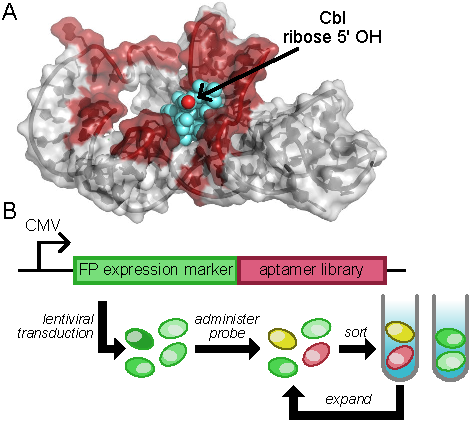
\includegraphics[width=\textwidth]{figures/aim2v2.pdf}

\end{centering}
\footnotesize
\caption{\label{figure:aim2}
A) Riboswitch sites for mutation (colored red) will be targeted based on potential contact with the linker and fluorophore, while the cobalamin (blue) binding site will be retained. (PDB: 4FRN, ref.\ \cite{JohnsonJrB12cofactorsdirectly2012)} B) RNA sequences will be screened in mammalian cells for brightness relative to a fluorescent protein control.
}
\end{wrapfigure}
%%%%%%%%%%%%%%%%%%%%%%%%%%%%%%%%%%%%%%%%%%%%%%%%%%%%%%%%%%%%%%%%%%%%%%%%%%%%%%%%

First, a library will be designed that varies the environment surrounding the cobalamin binding pocket (Figure \ref{figure:aim2}A). Through the guidance of Robert Batey (see Batey support letter), sites will be chosen to retain affinity for the cobalamin, yet maximize the distance between quencher and fluorophore upon binding \cite{JohnsonJrB12cofactorsdirectly2012}.
Next, a screen for fluorescence intensity in mammalian cells will be used to select bright riboswitch sequences.
A cellular screen for brightness is crucial because it ensures that the riboswitch aptamer maintains robust folding in a complex environment.
The Palmer lab is a leader in technologies for tool development in mammalian cells \cite{FiedlerDropletMicrofluidicFlow2017,DeanHighSpeedMultiparameterPhotophysical2015}.
This expertise will be leveraged for screening libraries of cobalamin riboswitches (Figure \ref{figure:aim2}B). Libraries of transcripts will first be transduced into mammalian cells using lentivirus at a low multiplicity of infection to ensure incorporation of a single library member per cell (a technique widely used in the Palmer lab).
The probe of interest will be administered, and cells will be sorted via fluorescence activated cell sorting (FACS, see Equipment document).
Cells that show elevated brightness relative to a fluorescent protein expression control will be binned.
In this way, libraries of up to one million members will be screened.
I will collect, culture, and resubject bright variants to sorting until only highly fluorescent cells remain. Sequences will be evaluated through high-throughput sequencing.

New sequences identified through this screen will undergo rigorous characterization of their biophysical and photophysical properties \textit{in vitro}. It will be important to characterize the extinction coefficient of each complex upon binding the RNA tag, as well as their quantum yields and photostability. The binding affinity for each probe-RNA combination will also be measured via isothermal titration calorimetry.
I will aim to retain K\textsubscript{D} values in the nanomolar range (the native riboswitch binds cobalamin at K\textsubscript{D} = 37 nM).
Such a value is important because it informs the probe dosage that will be necessary for imaging (and lower probe dosages will contribute less fluorescence background). Experiments to obtain these values are readily carried out in the Palmer Lab  \cite{ParkQuantitativeMeasurementCa22014,BraselmannDevelopmentriboswitchbasedplatform2017}.

Candidate probes that exhibit low background fluorescence, high signal induction, and high RNA affinity will be tested to determine the absolute level of turn-on fluorescence, and the minimum number of fluorophores that can be localized. To do this, $\upbeta$-actin mRNA will be tagged with one, two, or four repeats of the mutant riboswitch of interest in U2-OS cells through transient transfection. The cells will be imaged under conditions analogous to previous studies \cite{KatzMappingtranslationhotspots2016} using a TIRF microscope (see Equipment document). If puncta that appear to be single molecules are observed under these conditions, probe localization will be verified via fluorescence in situ hybridization (FISH) following cell fixation. If puncta are not visible in the initial TIRF images, cells will be treated with arsenite to induce the formation of stress granules (SGs) that also contain the protein G3BP1 \cite{ZurlaCharacterizingmRNAInteractions2011,JainATPaseModulatedStressGranules2016,NellesProgrammableRNATracking2016}.
G3BP1 can be tagged with the Halo-tag, and subsequently labeled with an orthogonal fluorophore to evaluate co-localization. A check of direct mRNA location can then be carried out with FISH.
This is a technique that the Palmer lab has previously used successfully to test Riboglow probes \cite{BraselmannDevelopmentriboswitchbasedplatform2017}.

To quantify our ability to resolve single mRNA molecules, we will utilize single-molecule FISH (smFISH) imaging to correlate RNA count with Riboglow signal \cite{MuellerFISHquantautomaticcounting2013}. This same method was recently used to quantify the sensitivity of an improved MS2 system \cite{TutucciimprovedMS2system2018}.
%If initial studies prove successful, we will attempt to image lncRNA \textit{SNHG5} in the cytosol of colorectal carcinoma (HCT116) cells, coupled with smFISH for verification \cite{DamasSNHG5promotescolorectal2016}.
%Studies involving imaging of lncRNA will be carried out under the supervision of Professor John Rinn, an expert in lncRNA (see Rinn support letter).

\textbf{Expected Outcomes and alternate approaches:}\\
To attain single-molecule resolution with Riboglow, the probes synthesized in Aim 1 will be screened with libraries of riboswitch mutants \textit{in cellulo}, targeting a 50-fold fluorescence turn-on. Cells containing bright mutants will be sorted via FACS and analyzed. Library hits will be characterized \textit{in vitro}, and tested via established assays for single-molecule localization \textit{in cellulo}.
%Probes that are successful in our model systems will be used to image long noncoding RNA under the supervision of Professor John Rinn.
While screening for high fluorescence in cells via FACS is the most efficient way to ensure robust turn-on, an alternative approach could involve alternating a screen for binding via \textit{in vitro} selection (see aim 3 for experimental detail) and in cellulo selection for fluorescence via FACS.
If single-molecule resolution is not observed in the library hits, additional riboswitches (over the four repeats already planned) can also be added to concentrate fluorescent signal. Even if 24 repeats are required, the construct will still be less than half the size of the MS2 system.

\subsubsection*{\underline{Aim 3.} Develop mutually orthogonal Riboglow probes for multicomponent imaging.}
% TODO include precedent:  \cite{HocineSinglemoleculeanalysisgene2013}
%%%%%%%%%%%%%%%%%%%%%%%%%%%%%%%%%%%%%%%%%%%%%%%%%%%%%%%%%%%%%%%%%%%%%%%%%%%%%%%%
%Aim 3: Multicomponent imaging
\begin{wrapfigure}[23]{L}{10cm}
  \vspace{-0.13in} % this is the happy medium between top of fig and bottom...
\begin{centering}
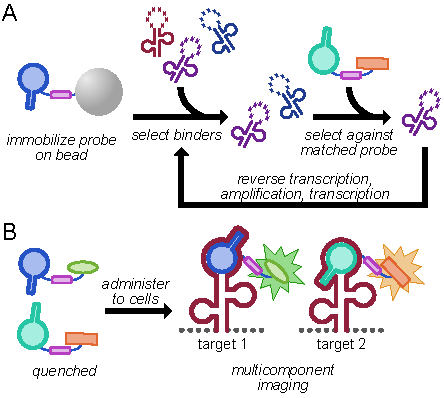
\includegraphics[width=\textwidth]{figures/aim3v2.pdf}
\end{centering}
\footnotesize
\caption{\label{figure:aim3}
A) SELEX will be used to screen for riboswitches that bind each cobalamin in a mutually-exclusive manner. B) Mutually orthogonal cobalamin analogs will enable multicomponent RNA imaging. Signal turn-on will only be observed in the presence of the matched pair.
}
\end{wrapfigure}
%%%%%%%%%%%%%%%%%%%%%%%%%%%%%%%%%%%%%%%%%%%%%%%%%%%%%%%%%%%%%%%%%%%%%%%%%%%%%%%%

The ability to track multiple RNA transcripts simultaneously would enable study of the interactions of RNA as they move throughout the cell. Upregulation of \textit{SNHG5} in colorectal cancer has been implicated in stabilization of a variety of mRNA in the cytoplasm that enable tumor survival \cite{DamasSNHG5promotescolorectal2016}. Direct hybridization of this lncRNA with mRNA protects transcipts from degradation, and enables translation, promoting disease states. Despite these implications, the spatiotemporal dynamics of lncRNA and their interacting partners have never been visualized in living cells, and thus their functions remain unknown. Localization of these lncRNA and their mRNA targets would shed light on these ``dark'' processes.

The modularity of the Riboglow platform is well suited to enable such an experiment, however mutually orthogonal riboswitch-probe pairs must first be identified. \textit{In vitro selection will enable identification of mutually-selective riboswitch-probe pairs for multicomponent RNA imaging} (Figure \ref{figure:aim3}B). \textit{To start, I will identify two orthogonal riboglow probes.}

Fortunately, screening for substrate selectivity is well-precedented in RNA engineering through systematic evolution of ligands by exponential enrichment (SELEX) \cite{MairalAptamersmoleculartools2008,ChoApplicationsAptamersSensors2009}.
In fact, \textit{de novo} aptamers have already been developed for cobalamin and a few of its analogs via SELEX \cite{LorschvitroselectionRNA1994}. This important precedent shows that even small changes to the structure of the cobalamin can be distinguished by engineered RNA, indicating that no additional changes will need to be made to the cobalamin structure apart from those constructs already proposed above. However, to improve our chances at identifying mutually-orthogonal probes, we will begin by screening probes that contain each of the two linker attachment points (Aim 1) to maximize structural differences at the cobalamin center.

Importantly, our selection experiments will not start from a completely randomized sequence of nucleic acids. It will be crucial to retain the original fold (and thus \textit{in cellulo} stability) of the native riboswitch. RNA biosensors developed in this way are known to have increased stability relative to aptamers selected \textit{de novo} \cite{PorterRecurrentRNAmotifs2017}.
Additionally, the brightest probe sequences identified in Aim 2 will be retained to preserve the bound conformation of the linker and fluorophore as much as possible.
The design of the starting RNA libraries, and subsequent selection experiments will be carried out under the supervision of Professor Robert Batey (see Batey letter of support), an expert in SELEX and RNA engineering \cite{TrauschChapterThreeDesign2015,PorterRecurrentRNAmotifs2017}.
Libraries will target bases known to participate in contacts with the cobalamin small molecule \cite{JohnsonJrB12cofactorsdirectly2012,PorterRecurrentRNAmotifs2017}.
The selection will be carried out as shown in Figure \ref{figure:aim3}A. Briefly, the cobalamin probe of interest will be immobilized on a bead via the same linker that will be used in the final construct.
The synthetic library of riboswitches will be incubated with the beads, and unbound sequences will be rinsed away.
Riboswitches that bind selectively will be collected and amplified (via reverse transcription, PCR amplification, and transcription) to undergo another round of selection (for a total of 7-10 rounds).
In subsequent rounds, the stringency of the screen will be increased via additional washes and reduction of RNA concentration.
In the final 2-3 rounds of selection, a counterselection will be conducted to ensure orthogonality with our other synthetic probes (Figure \ref{figure:aim3}A). In this way, the probe (or probes) intended to be orthogonal to the construct under selection will wash away any riboswitches that do not bind selectively.
Riboswitches will be deep sequenced to identify library convergence and optimal clones \cite{PorterRecurrentRNAmotifs2017}. This process will be repeated for each probe of interest, with counterselections against each other probe that is intended for multiplexed use.
% TODO make a point here about how unnatural ligand architectures will help reduce off-target fluorescence.

Mutually-orthogonal probes identified through the \textit{in vitro} selection will be verified in a similar fashion as described in Aim 2. Probe extinction coefficient, quantum yield, photostability, and binding affinity will be characterized \textit{in vitro}. Probes will also be independently verified \textit{in cellulo} via the $\upbeta$-actin fusion assay described in Aim 2 to ensure signal induction was retained.

Once a robust pair of Riboglow probes is identified, a lncRNA will be imaged interacting with a putative binding partner mRNA as a proof-of-concept.
Studies involving imaging of lncRNA will be carried out under the supervision of Professor John Rinn, an expert in lncRNA (see Rinn support letter).
First, \textit{SNHG5} will be tagged with one of our riboswitches and imaged in the cytosol of colorectal carcinoma (HCT116) cells, coupled with smFISH for verification.
Known phenotypic checks will be used to ensure that \textit{SNGH5} behaves normally upon tagging \cite{DamasSNHG5promotescolorectal2016}. % From damas paper: To investigate an impact of SNHG5 on survival, CRC cell lines were stained for cleaved Caspase-3 protein and analysed by flow cytometry, which revealed a strong induction of apoptosis in both HCT116, CACO-2 and DLD-1 cells (Fig. 2c, top).

Next, our multicomponent Riboglow platform will be used to image \textit{SNGH5} interacting with mRNA. \textit{SNGH5} has been shown to promote colorectal cancer survival through base pairing in the 3'-UTR of mRNA that promote tumor growth \cite{DamasSNHG5promotescolorectal2016}.
\textit{SPATS2}, \textit{PTRM1}, and \textit{GLE1} have been identified as interacting partners. To test whether these interactions can be detected, we will tag these three transcripts (one at a time) with an orthogonal riboswitch, and image them in living HCT116 cells alongside the tagged \textit{SNGH5}.
To further study these interactions, \textit{SNGH5} will be both overexpressed (via transient expression) and knocked down (via RNA interference), which has been shown to increase and decrease, respectively, the levels of interacting transcripts \cite{DamasSNHG5promotescolorectal2016}.
An additional check for localization will be made through fluorescent tagging of \textit{STAU1}, a protein that binds to the 3'-UTR of mRNA and mediates their degradation \cite{ParkEonyoungStaufenmediatedmRNA2013}. Single molecule FISH will provide a final check of probe selectivity.

% TODO talk about checks for retained (single molecule) sensitivity here. if some sensitivity lost, can rescreen for brightness.

% Once mutually-selective Riboglow probes are identified, simultaneous detection of two transcripts will be attempted (Figure \ref{figure:aim3}B). In addition to $\upbeta$-actin mRNA stress granule localization, small nuclear RNA (snRNA) U1 will be labeled and visualized in U-bodies. Imaging of U1 in U-bodies is a second system that the Palmer lab has already used to test Riboglow probes \cite{BraselmannDevelopmentriboswitchbasedplatform2017}. In this assay, snRNA U1 is fused with the riboswitch of interest and transfected into cells. Upon treatment with Thapsigargin, U1 is sequestered to U-bodies in the nucleus and cytosol \cite{HuttenroleCajalbodyassociatedSUMO2014}. Marker protein survival motor neuron (SMN) is also known to localize to these structures, and can be tagged with a fluorescent protein or Halo-tag for co-localization.

% To test multicomponent labeling, cells will be cotransfected with two orthogonal riboswitches. One labeling $\upbeta$-actin mRNA, and the other fused to snRNA U1. The cells would then be treated with arsenite or Thapsigargin, and a mixture of both cobalamin probes would be bead loaded. Upon treatment with arsenite, only the first would be expected to be visualized in the stress granules that form, while treatment of Thapsigargin should only give puncta with signal for the second probe.

\textbf{Expected Outcomes and alternate approaches:}
To develop multicomponent Riboglow, \textit{in vitro} selection will identify orthogonal riboswitch-probe pairs through a series of selections and counterselections.
Following characterization \textit{in vitro}, probes will be tested for multiplexed imaging of lncRNA-mRNA interactions \textit{in cellulo}. It is possible that the \textit{in vitro} selection will result in a loss of fluorescence turn-on. If this is the case, riboswitch sequences will be resubjected to the \textit{in cellulo} fluorescence intensity screen described in Aim 2.
% AMY Again you can emphasize that you can itterate SELEX and cellular screen to maximize chances of identifying high affinity and orthogonal (SELEX) probes / aptamer pairs that have robust turn on in cells (cellular screen).
Additionally, it may be difficult for the riboswitch to differentiate probes with similar cobalamin-linker structures. If the SELEX screen does not yield well-resolved pairs, additional steric bulk can be added to to the cobalamin (at either the 5' OH of the ribose, or the axial position of the cobalt), to aid in differentiation \cite{ChrominskiVitaminB12Derivatives2014}.

These studies will provide the first glimpse into the real-time behavior of lncRNA \textit{SNGH5} and its interacting partners. With new tools in the RNA imaging toolkit, we will be able to ask new questions about the little understood biomolecule that accounts for half of all cellular transcription.
% TODO discuss what was accomplished in each aim and wrap up. maybe dicuss future implications?

%%% Local Variables: ***
%%% mode: latex ***
%%% TeX-master: "Research_and_SA.tex" ***
%%% End: ***
